\documentclass[11pt]{article}
%%%%%%%%% options for the file macros.tex

\def\showauthornotes{1}
\def\showkeys{0}
\def\showdraftbox{0}
% \allowdisplaybreaks[1]


\usepackage{amsmath, ulem, amssymb, amsfonts, hyperref, amsthm, listings, tcolorbox, bbm, xifthen, soul, mathtools}
\usepackage[margin=1in]{geometry}
\usepackage[linesnumbered,lined,boxed,commentsnumbered, ruled]{algorithm2e}
\hypersetup{
    colorlinks=true,
    linkcolor=blue,
    filecolor=magenta,      
    citecolor=magenta,      
    urlcolor=cyan,
}
\usepackage[
    backend=biber,
    style=alphabetic,
    sorting=ynt,
    backref=true
]{biblatex}
\usepackage[shortlabels]{enumitem}
\usepackage{cleveref}

\newtheorem{theorem}{Theorem}[section]
\newtheorem{lemma}[theorem]{Lemma}
\newtheorem{corollary}[theorem]{Corollary}
\newtheorem{claim}[theorem]{Claim}
\newtheorem{fact}[theorem]{Fact}
\newtheorem{open-problem}[theorem]{Open Problem}

\theoremstyle{definition}

\newtheorem{definition}[theorem]{Definition}
\newtheorem{example}[theorem]{Example}

\newtheorem{remark}{Remark}
\newtheorem{question}{Question}

\newcommand{\V}[1]{\mathbf{#1}\ignorespaces}
\renewcommand\AA{\boldsymbol{\mathit{A}}}
\newcommand\LL{\boldsymbol{\mathit{L}}}
\newcommand\MM{\boldsymbol{\mathit{M}}}
\newcommand\II{\boldsymbol{\mathit{I}}}
\newcommand\JJ{\boldsymbol{\mathit{J}}}
\newcommand\KK{\boldsymbol{\mathit{K}}}

\newcommand{\ab}[1]{\langle #1 \rangle}
\renewcommand{\subset}{\subseteq}
\newcommand{\dsquare}{\mathbin{\raisebox{.2ex}{
    \hspace{-.4em}$\bigcirc$\hspace{-.75em}{\rm s}\hspace{.15em}}}}
\newcommand{\from}{\overset{R}{\leftarrow}}
\newcommand{\1}{\mathbbm{1}}

\DeclareMathOperator{\USTCON}{USTCON}
\DeclareMathOperator{\STCON}{STCON}
\allowdisplaybreaks

\usepackage{tikz}

\usepackage[
    backend=biber,
% giveninits=true,
% natbib=true,
    style=alphabetic,
    url=false, 
 %   doi=true,
    hyperref,
    backref=true,
    backrefstyle=none,
    maxbibnames=10,
    sortcites
]{biblatex}
\addbibresource{papers.bib}

%%%%%%%%% Authornotes
\newcommand{\Snote}{\Authornote{S}}

\newenvironment{tight_enumerate}{
\begin{enumerate}
 \setlength{\itemsep}{2pt}
 \setlength{\parskip}{1pt}
}{\end{enumerate}}
\newenvironment{tight_itemize}{
\begin{itemize}
 \setlength{\itemsep}{2pt}
 \setlength{\parskip}{1pt}
}{\end{itemize}}


\renewcommand\vec{\V}
\newcommand\itxt[1]{\intertext{\indent#1}}

\addbibresource{refs.bib}

%%%%%%%%%%%%%%%%%%%%%%%%%

\begin{document}

\newcommand{\coursenum}{{CSC 2421H}}
\newcommand{\coursename}{{Graphs, Matrices, and Optimization}}
\newcommand{\courseprof}{Sushant Sachdeva}

\lecturetitle{1}{Introduction}{Dmitry Paramonov}{10 Sep 2018}

\section{Introduction to the course}

\subsection{Goal}
\label{sec:goal}

Graph algorithms have been a mainstay of algorithms since the
foundation of computer science. The notion of polynomial time
efficiency (the class \p) was defined in the context of the first
algorithm for matchings in general graphs. You must have seen some
graph algorithms in your undergraduate algorithms class.

When you think of algorithms on graphs, you probably think of BFS /
DFS -- or more broadly combinatorial algorithms. However, there is
another approach to designing algorithms on graphs -- one that's based
on matrices and continuous optimization. This approach was first taken
for graph partitioning by Cheeger's inequality~\cite{AlonM85}, which
blossomed into the field of `Spectral graph theory'. Another thread in
this direction has been to incorporate numerical algorithms, and
continuous optimization methods, that has become very popular over the
last one and half decades since the work of Spielman and
Teng~\cite{SpielmanT04}.

The goal of this course will be to introduce you to the fundamentals
of these fields, to make you familiar with the tools and techniques
used here, and to equip you to be able to follow the latest research
in this area.

\subsection{Pre-requisites}
Officially, the pre-requisites are undergraduate algorithms, linear
algebra, probability, and some basic vector calculus. However, most
importantly of all, I expect mathematical maturity. This course will
be theoretical, and very mathematical in nature. We will prove several
theorems, and give guarantees for our algorithms.

This is an advanced graduate course, so I expect that there will be
some mathematical background that you will not be aware of, I expect
you to read to make up for that background. Sometimes, I will point
you to material that I expect you to read before coming to class. I
expect the material to be less than 2 hrs of reading per week. If you
miss reading them, it might be hard for you to follow or appreciate
what I'm doing in class. At the same time, I will try to make my
lectures only refer to the background material in a black-box manner.

If you want to get a sense of the level of the material, take a look
at the lecture notes for my course CSC 2421H last year. The material
will be substantially different but the level and the flavor of the
material covered will be similar.

\subsection{Logistics}
\begin{tight_itemize}
\item Monday 3--5pm, short break @4pm $\le 5$ mins
\item Location: SS 2101
\item Office hours: by appointment, feel free to catch me after
  lectures
\item Email: sachdeva@cs.toronto.edu
\item No class on Oct 8 (reading week)
\end{tight_itemize}

\subsection{Grading}
\label{sec:grading}
\begin{tight_itemize}
\item 20\% scribe note : Scribing one lecture
\item 30\% grade : Take home mid-term. 
\item Post mid-term, you will be picking a paper(s) related to the
  course and reading it thoroughly. You will be expected to deliver a
  presentation on the paper, and prepare lecture-notes based on it.
\item 50\% grade : Paper presentation + making notes for the paper(s)
\end{tight_itemize}

\subsection{Outline of the Course}
Here is a rough plan for the course. WARNING: This is a tentative
plan, and subject to change.
\begin{tight_enumerate}
\item Graphs, and basic matrices
  \begin{tight_itemize}
  \item Eigenvalues
  \item Connections to random walks, conductance and mixing time
  \item Cheeger's inequality
  \end{tight_itemize}
\item Graph Sparsification
  \begin{tight_itemize}
  \item Matrix concentration bounds
  \item Effective-resistance / leverage scores
  \item Sparsification by leverage score sampling
  \end{tight_itemize}
\item Laplacian Solvers
  \begin{tight_itemize}
  \item Gradient descent / Conjugate gradient
  \item Preconditioning
  \item A near-linear time solver
  \end{tight_itemize}
\item Optimization on graphs
  \begin{tight_itemize}
  \item Max-flow as linear program
  \item Solving linear program approximately via continuous methods
  \end{tight_itemize}
\end{tight_enumerate}

\section{Graphs and Basic Matrices}
\subsection{Introduction to Graphs}
Any discussion of graphs must necessarily start with a definition of a graph.
\begin{definition}
A \emph{graph} is a pair of sets $G=\paren{V,E}$.
$V$ is the set of \emph{vertices}, and $E$ is a set of \emph{edges}.
\end{definition}

For this course, the assumption will be an undirected graph.
Thus, $E$ is a set of unordered pairs of vertices.

In common practice, there are many examples of graphs.
Friendships could be modelled as a graph,
with people serving as vertices
and edges representing whether they are friends or not.
The Internet can be modelled as a graph,
wherein individual computers are vertices
and edges are network connections.

However, in this course,
the focus will be on a more general case,
with abstract vertices and edges.

For this purpose, vertices will usually, unless otherwise stated,
be assumed to be of the form $V=\sqparen{n}=\set{1,\ldots,n}$.
$n$ is usually used to denote the number of vertices in a graph,
while $m=\abs{E}$ is used to denote the number of edges.

As a simple example of a graph, consider the ring graph.
The edge set is of the form
$E=\set{\paren{i,i+1}:i\in\sqparen{n-1}}\cup\set{\paren{n,1}}$.
In this case, the vertices are connected in a cycle,
appearing as a ring.

\begin{center}
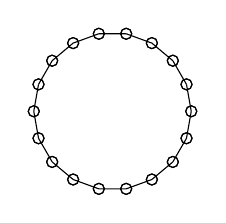
\begin{tikzpicture}[c/.style={insert path={circle[radius=2pt]}}]
\foreach \t in {-40,-20,...,300} {
    \draw (\t:1)[c] -- (\t+20:1)[c];
}
\end{tikzpicture}
\end{center}

This can also be modified into the path graph.
In this case, the edge set is just the first,
$E=\set{\paren{i,i+1}:i\in\sqparen{n-1}}$.

\begin{center}
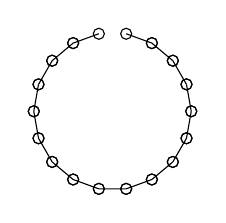
\begin{tikzpicture}[c/.style={insert path={circle[radius=2pt]}}]
\foreach \t in {100,120,...,420} {
    \draw (\t:1)[c] -- (\t+20:1)[c];
}
\end{tikzpicture}
\end{center}

Another notable example is a hypercube.
The vertex set for a hypercube is $V=\set{0,1}^{k}$,
the set of $k$-length strings of $0$'s and $1$'s.
The set of edges is then the set of all pairs of vertices $\paren{x,y}$
such that $x$ and $y$ differ in exactly one coordinate.
The hypercubes for $k=1,2,3$ are sketched below.
\begin{center}
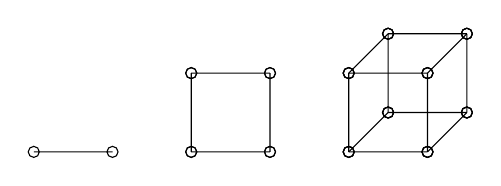
\begin{tikzpicture}[c/.style={insert path={circle[radius=2pt]}}]
\draw (0,0)[c] -- (1,0)[c];
\foreach \x in {2,3} {%
    \draw (\x,0)[c] -- (\x,1)[c];
}
\foreach \y in {0,1} {%
    \draw (2,\y)[c] -- (3,\y)[c];
}
\foreach \x in {4,5} {%
    \foreach \y in {0,1} {%
        \draw (\x,\y)[c] -- (\x+0.5,\y+0.5)[c];
    }
}
\foreach \x in {4,5} {%
    \foreach \z in {0,0.5}{%
        \draw (\x+\z,0+\z)[c] -- (\x+\z,1+\z)[c];
    }
}
\foreach \y in {0,1}{%
    \foreach \z in {0,0.5}{%
        \draw (4+\z,\y+\z)[c] -- (5+\z,\y+\z)[c];
    }
}
\end{tikzpicture}
\end{center}

Another useful graph is the $n$-star,
a graph where $E=\set{\paren{n,i}:i\in\sqparen{n-1}}$.
Here, all vertices are connected to one specific vertex,
with no other edges in the graph.

\begin{center}
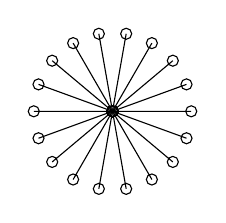
\begin{tikzpicture}[c/.style={insert path={circle[radius=2pt]}}]
\foreach \t in {-40,-20,...,300} {
    \draw (\t:1)[c] -- (0,0)[c];
}
\end{tikzpicture}
\end{center}

And a complete graph is a graph where all possible edges occur,
discounting self-loops, such that $E=\set{\paren{i,j}:i\neq j}$.
This is usually denoted $K_n$ for $n$ vertices.

\begin{center}
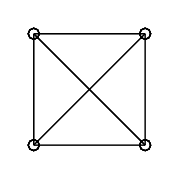
\begin{tikzpicture}[c/.style={insert path={circle[radius=2pt]}}]
\foreach \t in {-45,45,...,225} {
    \foreach \u in {-45,45,...,225} {
        \draw (\t:1)[c] -- (\u:1)[c];
    }
}
\end{tikzpicture}
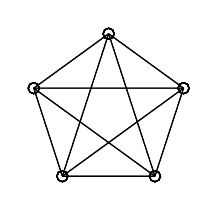
\begin{tikzpicture}[c/.style={insert path={circle[radius=2pt]}}]
\foreach \t in {18,90,...,306} {
    \foreach \u in {18,90,...,306} {
        \draw (\t:1)[c] -- (\u:1)[c];
    }
}
\end{tikzpicture}
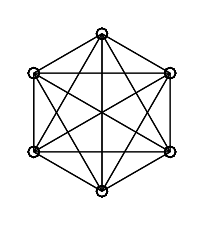
\begin{tikzpicture}[c/.style={insert path={circle[radius=2pt]}}]
\foreach \t in {-30,30,...,270} {
    \foreach \u in {-30,30,...,270} {
        \draw (\t:1)[c] -- (\u:1)[c];
    }
}
\end{tikzpicture}
\end{center}

\subsection{Matrix Represenation of Graphs}
For most purposes, algorithms to be run on graphs are run on computers.
Thus, we wish for an efficient way of representing it.
Matrices can be efficiently stored on a computer,
so representing a graph as a matrix would be convenient.

The most straightforward way to represent a matrix on a computer is an adjacency matrix.
This represents which vertices are adjacent.
\begin{definition}
An \emph{adjacency matrix} of a graph $G=\paren{V,E}$
is a matrix $\V{A}\in\rea^{V\times V}$ such that
$$\V{A}\paren{u,v}=\begin{cases}1,&\paren{u,v}\in E,\\
0,&\text{otherwise}.\end{cases}$$

A $1$ indicates that there is an edge between these vertices,
and a $0$ indicates that there isn't.
\end{definition}

This can be generalized for weighted graphs,
graphs with an associated weight function $w:E\to\rea$ by storing the weights.
$$\V{A}\paren{u,v}=\begin{cases}w\paren{u,v},&\paren{u,v}\in E,\\
0,&\text{otherwise}.\end{cases}$$

This representation can be used to quickly check connections between weights.
It allows for the testing of whether an edge is present in $O\paren{1}$ time.

However, adjacency matrices do not have any convenient mathematical properties.
Thus, while being a convenient storage format for graphs,
adjacency matrices don't actually allow for any advanced matrix-based analyses.

Another similar matrix is the degree matrix.
This uses the notion of the degree.
The degree of a vertex $v$, denoted by $\deg\paren{v}$
is the number of edges such that $v$ is an endpoint.
\begin{definition}
A \emph{degree matrix} of a graph $G=\paren{V,E}$
is a diagonal matrix $\V{D}\in\rea^{V\times V}$ such that
$$\V{D}\paren{u,v}=\begin{cases}0,&u\neq v,\\\deg\paren{u},&u=v.\end{cases}$$
\end{definition}

For this matrix, in the case of a weighted graph,
the values are the weighted degree,
the sum of the weights of all edges ending in this vertex.

However, this matrix also doesn't allow for convenient analysis.
In fact, the original graph cannot be reliably reconsructed from it.

Thus, another matrix is introduced, with more convenient properties.
\begin{definition}
The \emph{Laplacian} of a graph $G=\paren{V,E}$
is the unique symmetric matrix $\V{L}_{G}\in\rea^{V\times V}$ such that
$$\V{x}^{\top}\V{L}_{G}\V{x}
=\sum\limits_{\paren{u,v}\in E}\paren{\V{x}\paren{u}-\V{x}\paren{v}}^2.$$
\end{definition}

For a weighted graph, the quadratic terms are rescaled by the weight.
$$\vec{x}^{\top}\V{L}_{G}\vec{x}
=\sum\limits_{\paren{u,v}\in E}w\paren{u,v}
\paren{\vec{x}\paren{u}-\vec{x}\paren{v}}^2.$$

\newcommand\colvec[1]{\begin{pmatrix}#1\end{pmatrix}}

However, this only defines the Laplacian implicitly,
and we wish to find an explicit way of computing it.

Thus, let us begin with a single edge.
The graph $G_{uv}$ has some amount of vertices,
but has only one edge, between the vertices $u$ and $v$.
Let us attempt to compute the Laplacian for this, $\V{L}_{uv}$.
\begin{align*}
\vec{x}^{\top}\V{L}_{uv}\vec{x}
&=\paren{\vec{x}\paren{u}-\vec{x}\paren{v}}^2\\
&=\vec{x}\paren{u}^2+\vec{x}\paren{v}^2-2\vec{x}\paren{u}\vec{x}\paren{v}.\\
\vec{x}^{\top}\V{L}_{uv}\vec{x}
&=\sum\limits_{w,z\in V}\V{L}_{uv}\paren{w,z}
\vec{x}\paren{w}\vec{x}\paren{z}.\\
\itxt{Because we require the $\vec{x}\paren{u}^2$
and $\vec{x}\paren{v}^2$ coefficients to be $1$,
we see that the $u,u$ entries and $v,v$ entries must be $1$.
And therefore, the $u,v$ and $v,u$ entries must sum to $-2$.
But by symmetry, we can thus see their exact values.}
\therefore\V{L}_{uv}&=\colvec{1&-1\\-1&1}.\\
\itxt{We can also rewrite it another way.}
\text{Let }\vec{\chi}_{u}&\in\rea^n.\\
\vec{\chi}_{u}\paren{w}&=\begin{cases}1,&w=u,\\0,&\text{otherwise}.\end{cases}\\
\vec{x}^{\top}\V{L}_{uv}\vec{x}
&=\paren{\vec{x}\paren{u}-\vec{x}\paren{v}}^2\\
&=\paren{\paren{\vec{\chi}_u-\vec{\chi}_v}^{\top}\vec{x}}^2.\\
\itxt{We can thus expand the thing in the middle.}
\paren{\vec{\chi}_u-\vec{\chi}_v}\paren{w}
&=\begin{cases}1,&w=u,\\-1,&w=v,\\0,&\text{otherwise}.\end{cases}\\
\vec{x}^{\top}\V{L}_{uv}\vec{x}
&=\paren{\paren{\vec{\chi}_u-\vec{\chi}_v}^{\top}\vec{x}}^2\\
&=\paren{\paren{\vec{\chi}_u-\vec{\chi}_v}^{\top}\vec{x}}^{\top}
\paren{\paren{\vec{\chi}_u-\vec{\chi}_v}^{\top}\vec{x}}\\
&=\vec{x}^{\top}\paren{\vec{\chi}_u-\vec{\chi}_v}
\paren{\vec{\chi}_u-\vec{\chi}_v}^{\top}\vec{x}.\\
\V{L}_{uv}&=\paren{\vec{\chi}_u-\vec{\chi}_v}
\paren{\vec{\chi}_u-\vec{\chi}_v}^{\top}\\
&=\colvec{1\\-1}\colvec{1&-1}\\
&=\colvec{1&-1\\-1&1}.\\
\end{align*}

Thus, in the single edge case,
we can extract our $\V{L}_{uv}$ explicitly.
Note that this only concerns the submatrix involving $u$ and $v$.
For all other vertices, as they have no edges, all coefficients are $0$.

% Natural Quadratic Form Comment Goes Here
We can also find a more general case of the Laplacian.
Note that the quadratic form is necessarily linear in the edges.
Thus, we can rederive the full $\V{L}_G$ from that property.
\begin{align*}
\vec{x}^{\top}\V{L}_{G}\vec{x}&=\sum\limits_{\paren{u,v}\in E}
w\paren{u,v}\paren{\vec{x}\paren{u}-\vec{x}\paren{v}}^2\\
&=\sum\limits_{\paren{u,v}\in E}w\paren{u,v}
\paren{\vec{x}^{\top}\V{L}_{uv}\vec{x}}\\
&=\vec{x}^{\top}\paren{\sum\limits_{\paren{u,v}\in E}
w\paren{u,v}\V{L}_{uv}}\vec{x}.\\
\V{L}_{G}&=\sum\limits_{\paren{u,v}\in E}w\paren{u,w}\V{L}_{uv}.\\
\end{align*}

We also claim that the following is another definition of the Laplacian,
but the proof is left as an exercise to the reader.
$$\V{L}_{G}=\V{D}-\V{A}.$$

\subsection{The Spectral Theorem}
Now that we can represent our graphs as matrices,
the obvious question becomes as to what we can do with this.
Is there some information we can extract from it while it in matrix form
which we could not easily extract earlier?

It turns out that we can.
But to demonstrate this, we first need to cover the Spectral Theorem.
\begin{definition}
For a given matrix $\V{M}\in\rea^{n\times n}$,
$\vec{\psi}\in\rea^{n}$ is an eigenvector of $M$
with $\lambda\in\rea$ as an eigenvalue if $\V{M}\vec{\psi}=\lambda\vec{\psi}$,
under the condition that $\vec{\psi}\neq 0$.
\end{definition}

Note that not all matrices have eigenvalues or eigenvectors.
However, square symmetric matrices have very interesting properties,
which are given by the Spectral Theorem.
\begin{theorem}[Spectral Theorem]
If $\V{M}$ is a symmetric $n\times n$ matrix,
then there exist $\vec{\psi}_1,\ldots,\vec{\psi}_n\in\rea^n$
which are mutually orthonormal
and such that each is an eigenvector of $\V{M}$,
with eigenvalues $\lambda_1,\ldots,\lambda_n$, respectively.

Furthermore,
$$\V{M}=\sum\limits_{i}\lambda_{i}\vec{\psi}_{i}\vec{\psi}_{i}^{\top}.$$
\end{theorem}

Note that these eigenvalues are not necessarily distinct.
You can have duplicates.
But if you count them, taking into account multiplicity,
we see that there are $n$ total.

Furthermore, our orthonormal eigenvectors form a basis of the space,
so we can write any vector as a linear combination of them.

As an example, consider a matrix $\V{U}$,
with each column being a different $\vec{\psi}_i$.
$$\V{U}=\colvec{\vec{\psi}_1&\cdots&\vec{\psi}_n}.$$

Note that we thus get that $\V{U}^{\top}\V{U}=\V{I}_{n\times n}$, the identity.
And by properties of orthonormal matrices,
we get that $\V{U}\V{U}^{\top}=\V{I}_{n\times n}$
And we can thus rewrite $\V{M}$.
Let $\V{\Lambda}$ be the diagonal matrix
with $\lambda_1,\ldots,\lambda_n$ on the diagonal.
In that case, $\V{M}$ gets a very convenient representation.
$$\V{M}=\V{U}\V{\Lambda}\V{U}^{\top}.$$

We also know that $\lambda$ is an eigenvalue of $\V{M}$
if and only if $\det\paren{t\V{I}-\V{M}}=0$ has $\lambda$ as a solution.

% As a convention, we order our eigenvalues in non-decreasing order.

\subsection{Spectral Theorem on Graphs}
Now, let us apply the above on graphs.

Let us begin with a single edge.
\begin{align*}
\V{A}&=\colvec{0&1\\1&0}.\\
\V{D}&=\colvec{1&0\\0&1}.\\
\V{L}&=\colvec{1&-1\\-1&1}.\\
\itxt{We can now find eigenvectors for this.}
\V{L}\colvec{1\\1}&=\colvec{0\\0}.\\
\vec{\psi}_1&=\frac{1}{\sqrt{2}}\colvec{1\\1}.\\
\lambda_1&=0.\\
\itxt{From this, you can try to construct another one,
by taking an orthogonal vector.}
\vec{\psi}_2&=\frac{1}{\sqrt{2}}\colvec{1\\-1}.\\
\lambda_2&=2.
\end{align*}

You thus have an eigen-decomposition.
You can also find the latter one
just by recalling the $\vec{\chi}$ form of $\V{L}_{uv}$,
from which you can see that
$\V{L}_{uv}=\paren{\vec{\chi}_u-\vec{\chi}_v}
\paren{\vec{\chi}_u-\vec{\chi}_v}^{\top}$.
Thus, by starting from the final step of the Spectral Theorem,
we see that $\paren{\vec{\chi}_u-\vec{\chi}_v}$ must be an eigenvector,
which actually gives us exactly $\vec{\psi}_2$.

We can also try to calculate the decomposition of the complete graph.
\begin{align*}
\V{D}&=\colvec{n-1&0&\cdots&0\\0&n-1&\cdots&0\\
\vdots&\vdots&\ddots&\vdots\\0&0&\cdots&n-1}.\\
\V{A}&=\colvec{0&1&\cdots&1\\1&0&\cdots&1\\
\vdots&\vdots&\ddots&\vdots\\1&1&\cdots&0}.\\
\V{L}&=\V{D}-\V{A}\\
&=\colvec{n-1&-1&\cdots&-1\\-1&n-1&\cdots&-1\\
\vdots&\vdots&\ddots&\vdots\\-1&-1&\cdots&n-1}\\
&=n\V{I}-\colvec{1&1&\cdots&1\\1&1&\cdots&1\\
\vdots&\vdots&\ddots&\vdots\\1&1&\cdots&1}\\
\itxt{This latter matrix is usually denoted by $\V{J}$.}
&=n\V{I}-\V{J}\\
\itxt{We can also express this using the all-ones vector,
$\vec{\V{1}}\paren{v}=1\forall v\in V$.}
&=n\V{I}-\vec{\V{1}}\vec{\V{1}}^{\top}.\\
\end{align*}

Now, we can see that $\vec{\V{1}}\vec{\V{1}}^{\top}$
has 1 eigenvalue of $n$, as before,
and $n-1$ eigenvalues of $0$, since this is a matrix of rank $1$.

However, note that if $\lambda$ is an eigenvalue of $\V{M}$,
then $n-\lambda$ is an eigenvalue of $n\V{I}-\V{M}$, and vice versa.

And thus, $n\V{I}-\vec{\V{1}}\vec{\V{1}}^{\top}$
has $n-1$ eigenvalues of $n$ and $1$ eigenvalue of $0$.

Thus, we get the eigenvalues of $K_n$.

We also get some nice properties.
\begin{lemma}
For any Laplacian, the eigenvalues are all non-negative.
\end{lemma}
\begin{proof}
To see this, consider $\vec{\psi}_i$ and $\lambda_i$.
\begin{align*}
\V{L}\vec{\psi}_i&=\lambda_i\vec{\psi}_i\\
\vec{\psi}_i^{\top}\V{L}\vec{\psi}_i
&=\lambda_i\vec{\psi}_i^{\top}\vec{\psi}_i.\\
\itxt{We know by orthonormality that the vector product must be non-negative.}
\vec{\psi}_i^{\top}\vec{\psi}_i&\geq 0.\\
\itxt{But we also know by quadratic forms that the left side
must also be non-negative.}
\vec{\psi}_i^{\top}\V{L}\vec{\psi}_i&\geq 0.\\
\therefore\lambda_i&\geq 0.
\end{align*}
\end{proof}

\subsection{Conductance}
\begin{lemma}
Every Laplacian has an eigenvalue of $0$.
\end{lemma}
\begin{proof}
To see this, consider $\V{L}_{G}\vec{\V{1}}$.
We know that due to the quadratic form,
$$\vec{\V{1}}^{\top}\V{L}_{G}\vec{\V{1}}=0.$$

Alternatively, we can consider the expanded form.
\begin{align*}
\V{L}_{G}\vec{\V{1}}&=\paren{\V{D}-\V{A}}\vec{\V{1}}\\
&=0.\\
\end{align*}

This holds due to the sum over the rows in $A$
giving exactly the degree for that row.
\end{proof}

But we also get some interesting properties about connectivity.

\begin{lemma}
If $G$ is connected, and $\V{L}_{G}\vec{x}=0$ with $x\neq 0$,
then $\vec{x}$ must be of the form $c\vec{\V{1}}$.
\end{lemma}
\begin{proof}
\begin{align*}
\V{L}_{G}\vec{x}&=0.\\
\vec{x}^{\top}\V{L}_{G}\vec{x}&=0.\\
\sum\limits_{\paren{u,v}\in E}\paren{x\paren{u}-x\paren{v}}^2&=0.\\
\therefore\forall\paren{u,v}\in E,\quad x\paren{u}-x\paren{v}&=0.\\
\forall\paren{u,v}\in E,\quad x\paren{u}&=x\paren{v}.
\end{align*}
\end{proof}

In general, this means that every connected component
in your graph must have the same value,
with the entire graph getting the same value in the connected case.

This means that for a connected graph,
the only $0$-eigenvalued eigenvector is $\vec{\V{1}}$.
Which means that all other eigenvalues are non-zero.

\begin{lemma}
If $G$ has $k$ connected components,
then $\V{L}_{G}$ has $k$ eigenvectors with eigenvalue $0$,
and all others having a greater eigenvalue.
\end{lemma}
This is left as an exercise to the reader.

\printbibliography
\end{document}

%%% Local Variables:
%%% mode: latex
%%% TeX-master: t
%%% End:
